\subsubsection{KYMCO Agility Carry 50 E5}
\paragraph{Descripción general}
La \textbf{\textit{KYMCO Agility Carry 50 E5}} es el mejor modelo que podemos encontrar en el mercado, según las consideraciones descritas en el \refanexo{anexo:Ciclomotor Gasolina}, para reparto, las comodidades que ofrece tanto para el usuario como para desempeñar su tarea son únicas. Orientada a obtener la máxima funcionalidad, cuenta con una parrilla en la parte delantera y otra en la trasera, útil para los repartidores, ya que soporta hasta una carga de hasta 5 \glssymbol{kg}. 

\begin{figure}[h]
    \centering
    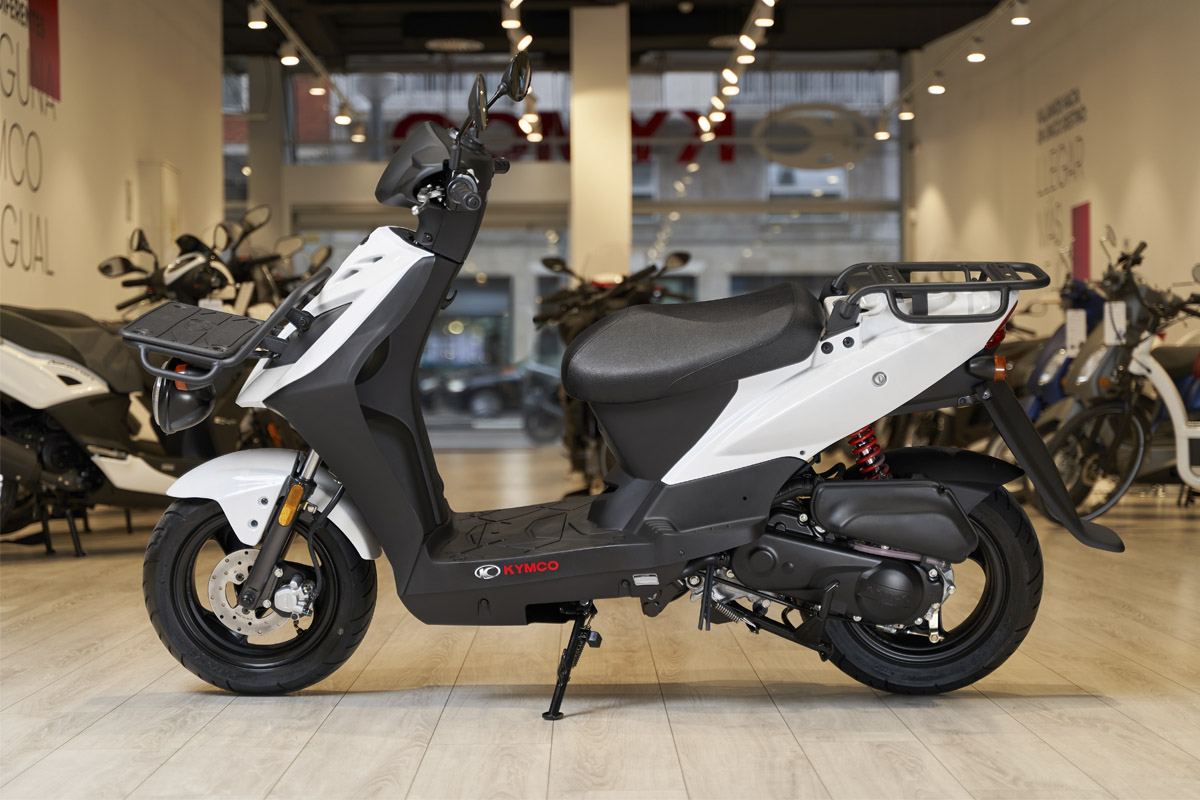
\includegraphics[scale = 0.25]{archivos/KYMCO agility carry.jpg}
    \caption{KYMCO Agility Carry 50 E5.}
    \label{fig:kymco agility carry}
\end{figure}

El motor de la \textbf{\textit{KYMCO Agility Carry 50 E5}} es de los más eficientes que hay en el mercado, se caracteriza por sus bajas emisiones y su poco consumo, tal y como se muestra en la \autoref{tab:comparacion de distintos modelos de ciclomotores de reparto}.

Además de las características que ofrece como equipo de reparto y del valor que añade a los usuarios, la empresa se ve beneficiada por su precio tan competitivo, sin lugar a dudas, su característica más destacable, ya que, por tan solo 1.999 \glssymbol{euro} la empresa puede contar con esta moto como parte de los activos. 

% \paragraph{Estudio del reparto.}
% Todos los cálculos asociados al reparto 
\paragraph{Mantenimiento y robustez}

Este modelo cuenta con un manual de usuario \cite{manualkymcociclomotor} en el que se específica el tratamiento que deben tener, los distintos elementos que componen la moto y la frecuencia con la que deben de cambiarse. 

Como se puede observar en la \autoref{fig:cambio kymco agility 50} el mantenimiento que necesita el ciclomotor no es excesivo, ya que el primer recambio de aceite es necesario después de 1000 \gls{km} o de 3 meses, lo cual nos conduce a la gran durabilidad y robustez con la que cuenta el ciclomotor.

La gran ventaja que ofrece el mantenimiento tardío radica en poder distribuirlos en el tiempo con mayor facilidad para evitar tener toda la flota en el taller y que se necesite de servicios auxiliares o de una segunda flota.

\begin{figure}[h]
    \centering
    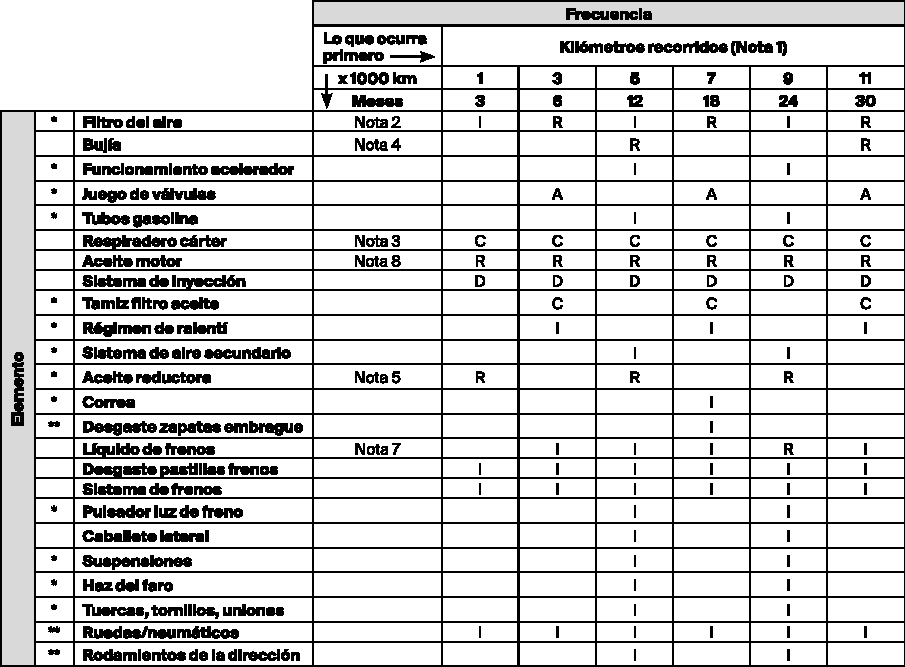
\includegraphics[scale = 1]{archivos/ManualUsuario_AgilityCity50.pdf}
    \caption{Tabla de mantenimiento del ciclomotor  KYMCO Agility Carry 50.}
    \label{fig:cambio kymco agility 50}
\end{figure}

\paragraph{Viabilidad económica}

En el \refanexo{Ciclomotor gasolina 50cc, KYMCO Agility Carry 50} se presentan una serie de cálculos relacionados con la viabilidad económica, en el que se concluye que este modelo es el más barato y el que requiere una menor inversión, cuyo dinero asciende a la cifra de 16.052,70 \glssymbol{euro} el primer año y los siguientes años 4.965,55 \glssymbol{euro}, según la \autoref{tab:Presupuesto motillo Peter}, por consiguiente esto nos da un total de 5 vehículos disponibles para el reparto, lo cual satisfará la demanda.

\paragraph{Conclusiones modelo}
Es el mejor ciclomotor con el que cuenta el mercado, está preparado para satisfacer todas las necesidades que se puedan presentar durante el desempeño de cualquier actividad de reparto, tiene un estilo moderno que combina con la imagen corporativa de cualquier empresa a una relación-calidad precio muy competitiva.